\documentclass[../ProgettoTecWeb2.tex]{subfiles}

\begin{document}
\section{Pagine interne}
	Con l'utilizzo dei motori di ricerca, la navigazione all'interno di un sito web non inizia sempre dall'home page ma può cominciare da una qualsiasi della pagine interne. Per tale motivo è utile al fine di garantire l'usabilità di un sito web soddisfare le 6W anche nelle pagine interne di un sito web.

	\subsection{Le pagine di recensioni, news, anteprime e speciali}
	Le pagine relative alle voci del menù ``Recensioni'', ``News'', ``Anteprime'' e ``Speciali'' sono pagine uguali alla home page: ogniuna di queste pagine difatti sembra avere il contenuto della home page filtrato solo per la categoria che rappresenta la pagine. Difatti nella home page troviamo queste tipologie di contenuti mescolati mentre ognuna delle voci contiene un'unica tipologia.
	L'unica differenza significatia riguarda lo ``slideshow'' presente nell'home page e non riproposto nelle altre pagine.

	\begin{figure} [H]
			\centering
			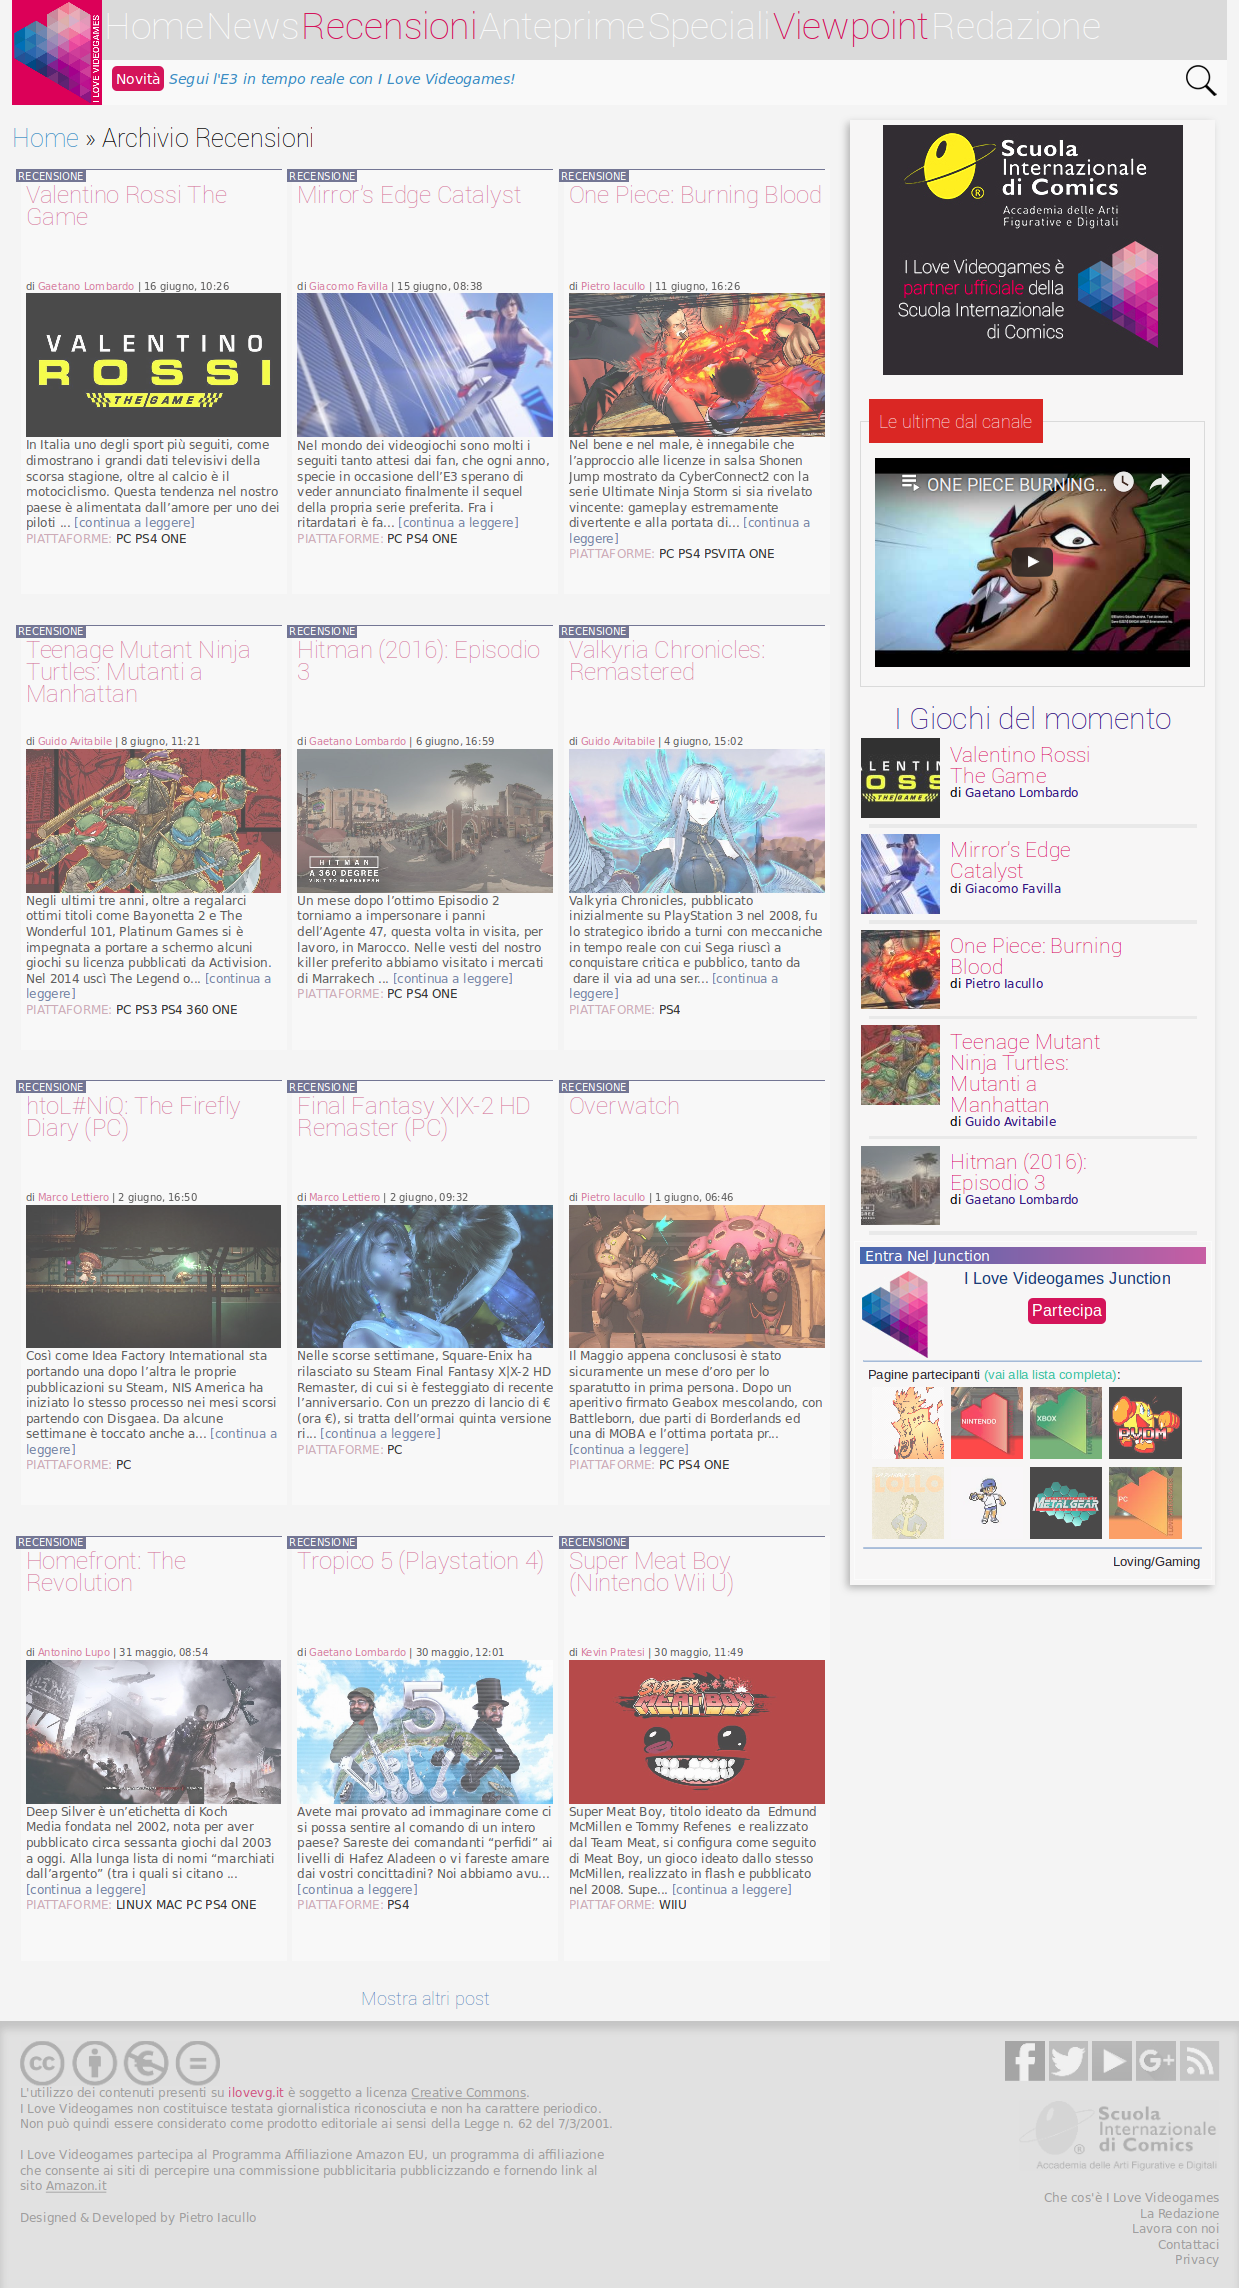
\includegraphics[scale=0.24]{img/RecensioniCompleta}
			\caption{Pagina con l'archivio delle recensioni}
	\end{figure}

	\begin{figure} [H]
			\centering
			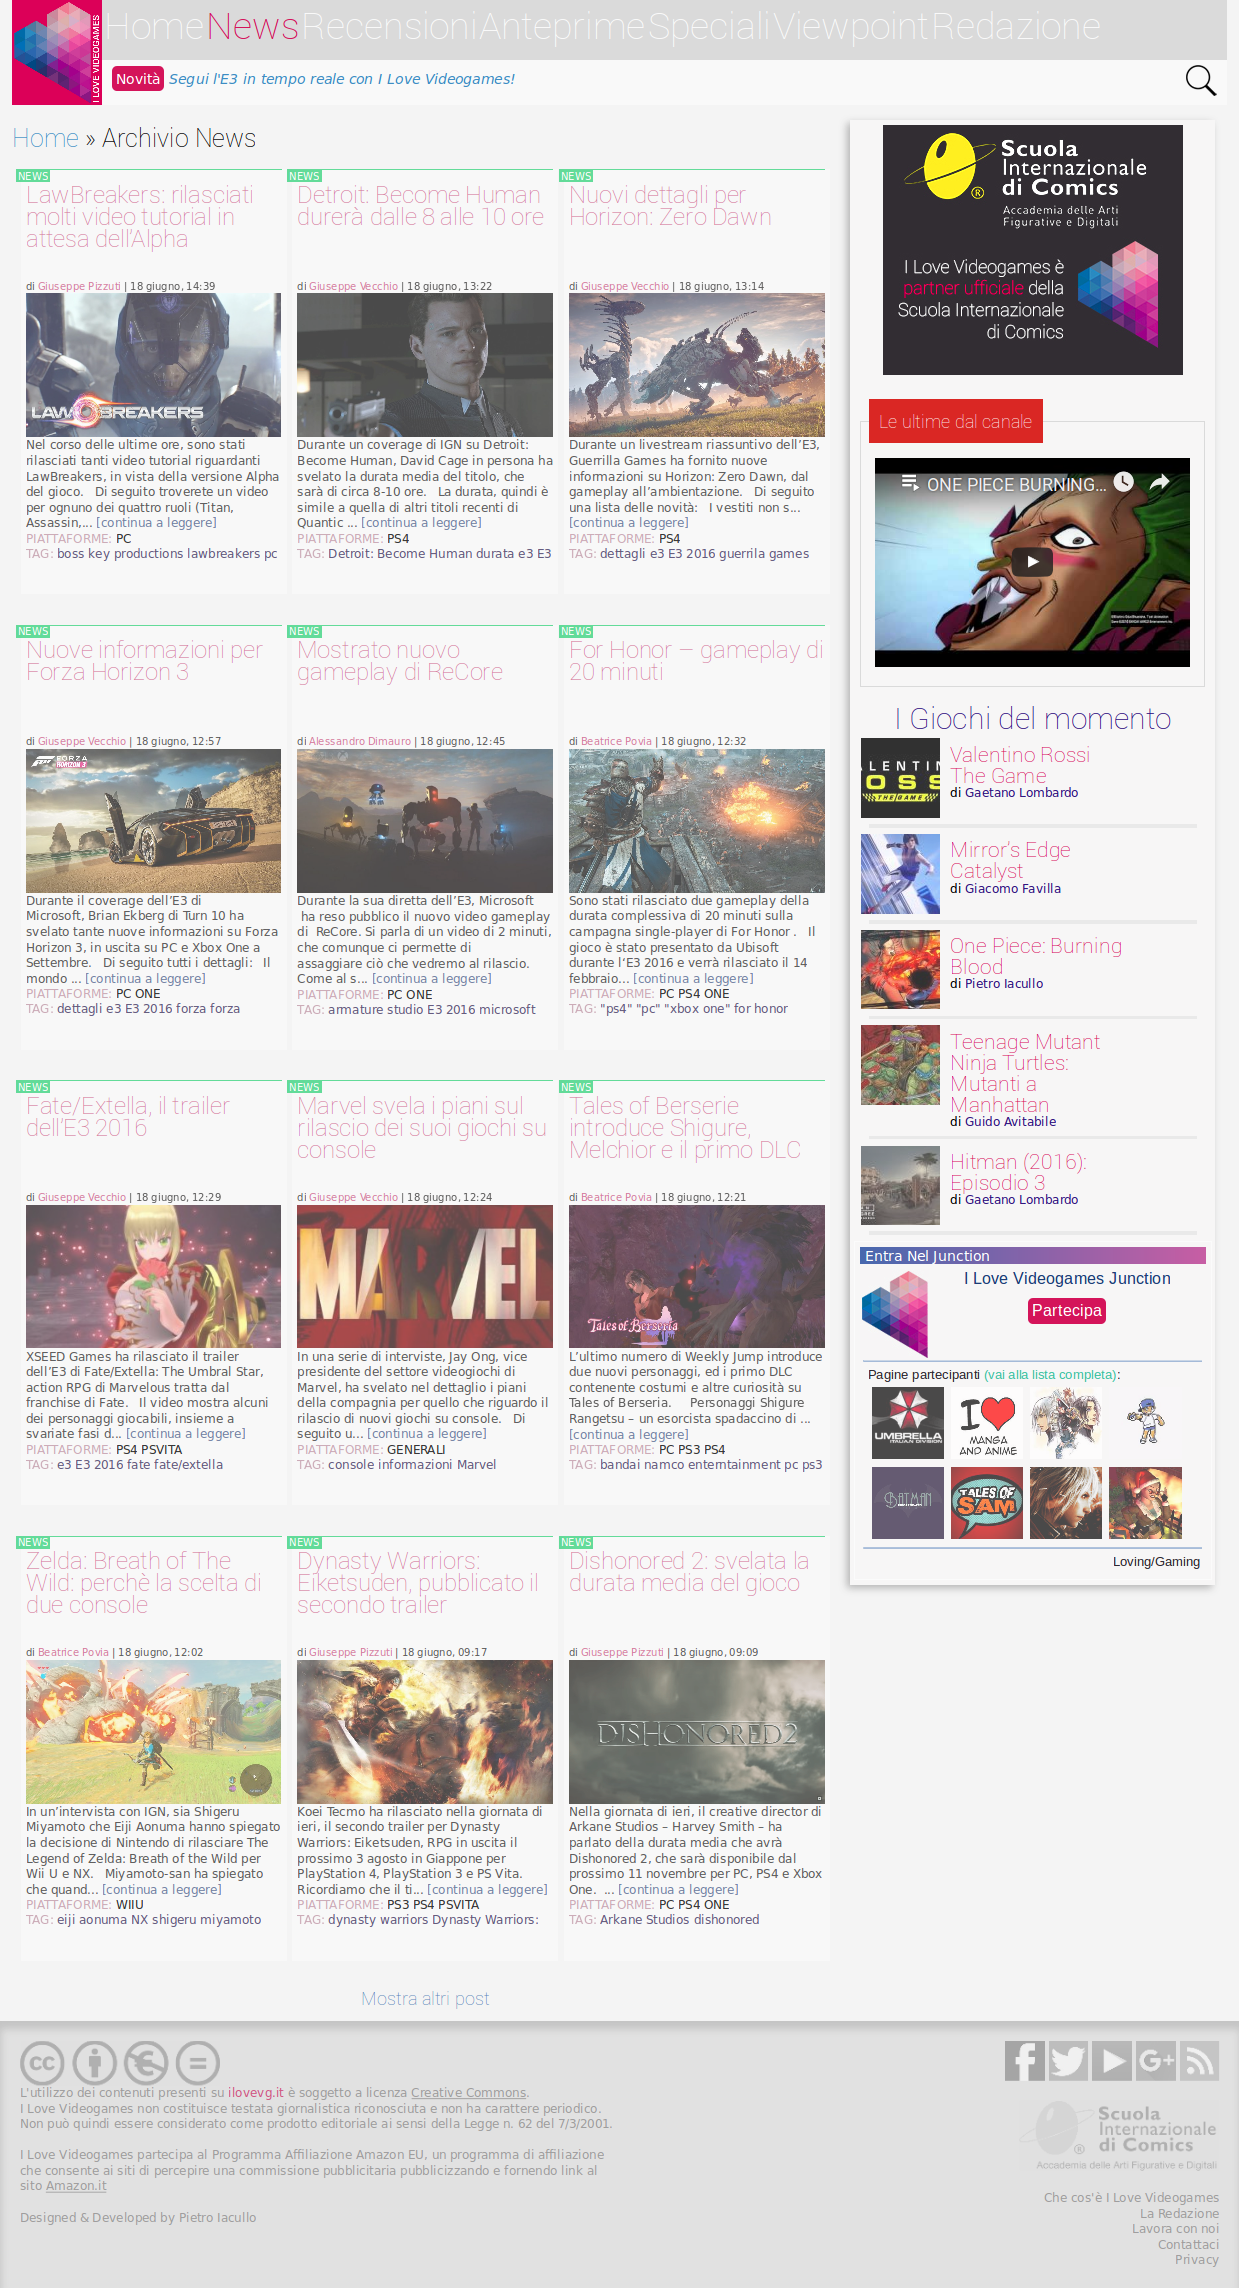
\includegraphics[scale=0.24]{img/NewsCompleta}
			\caption{Pagina con l'archivio delle news}
	\end{figure}

	\begin{figure} [H]
			\centering
			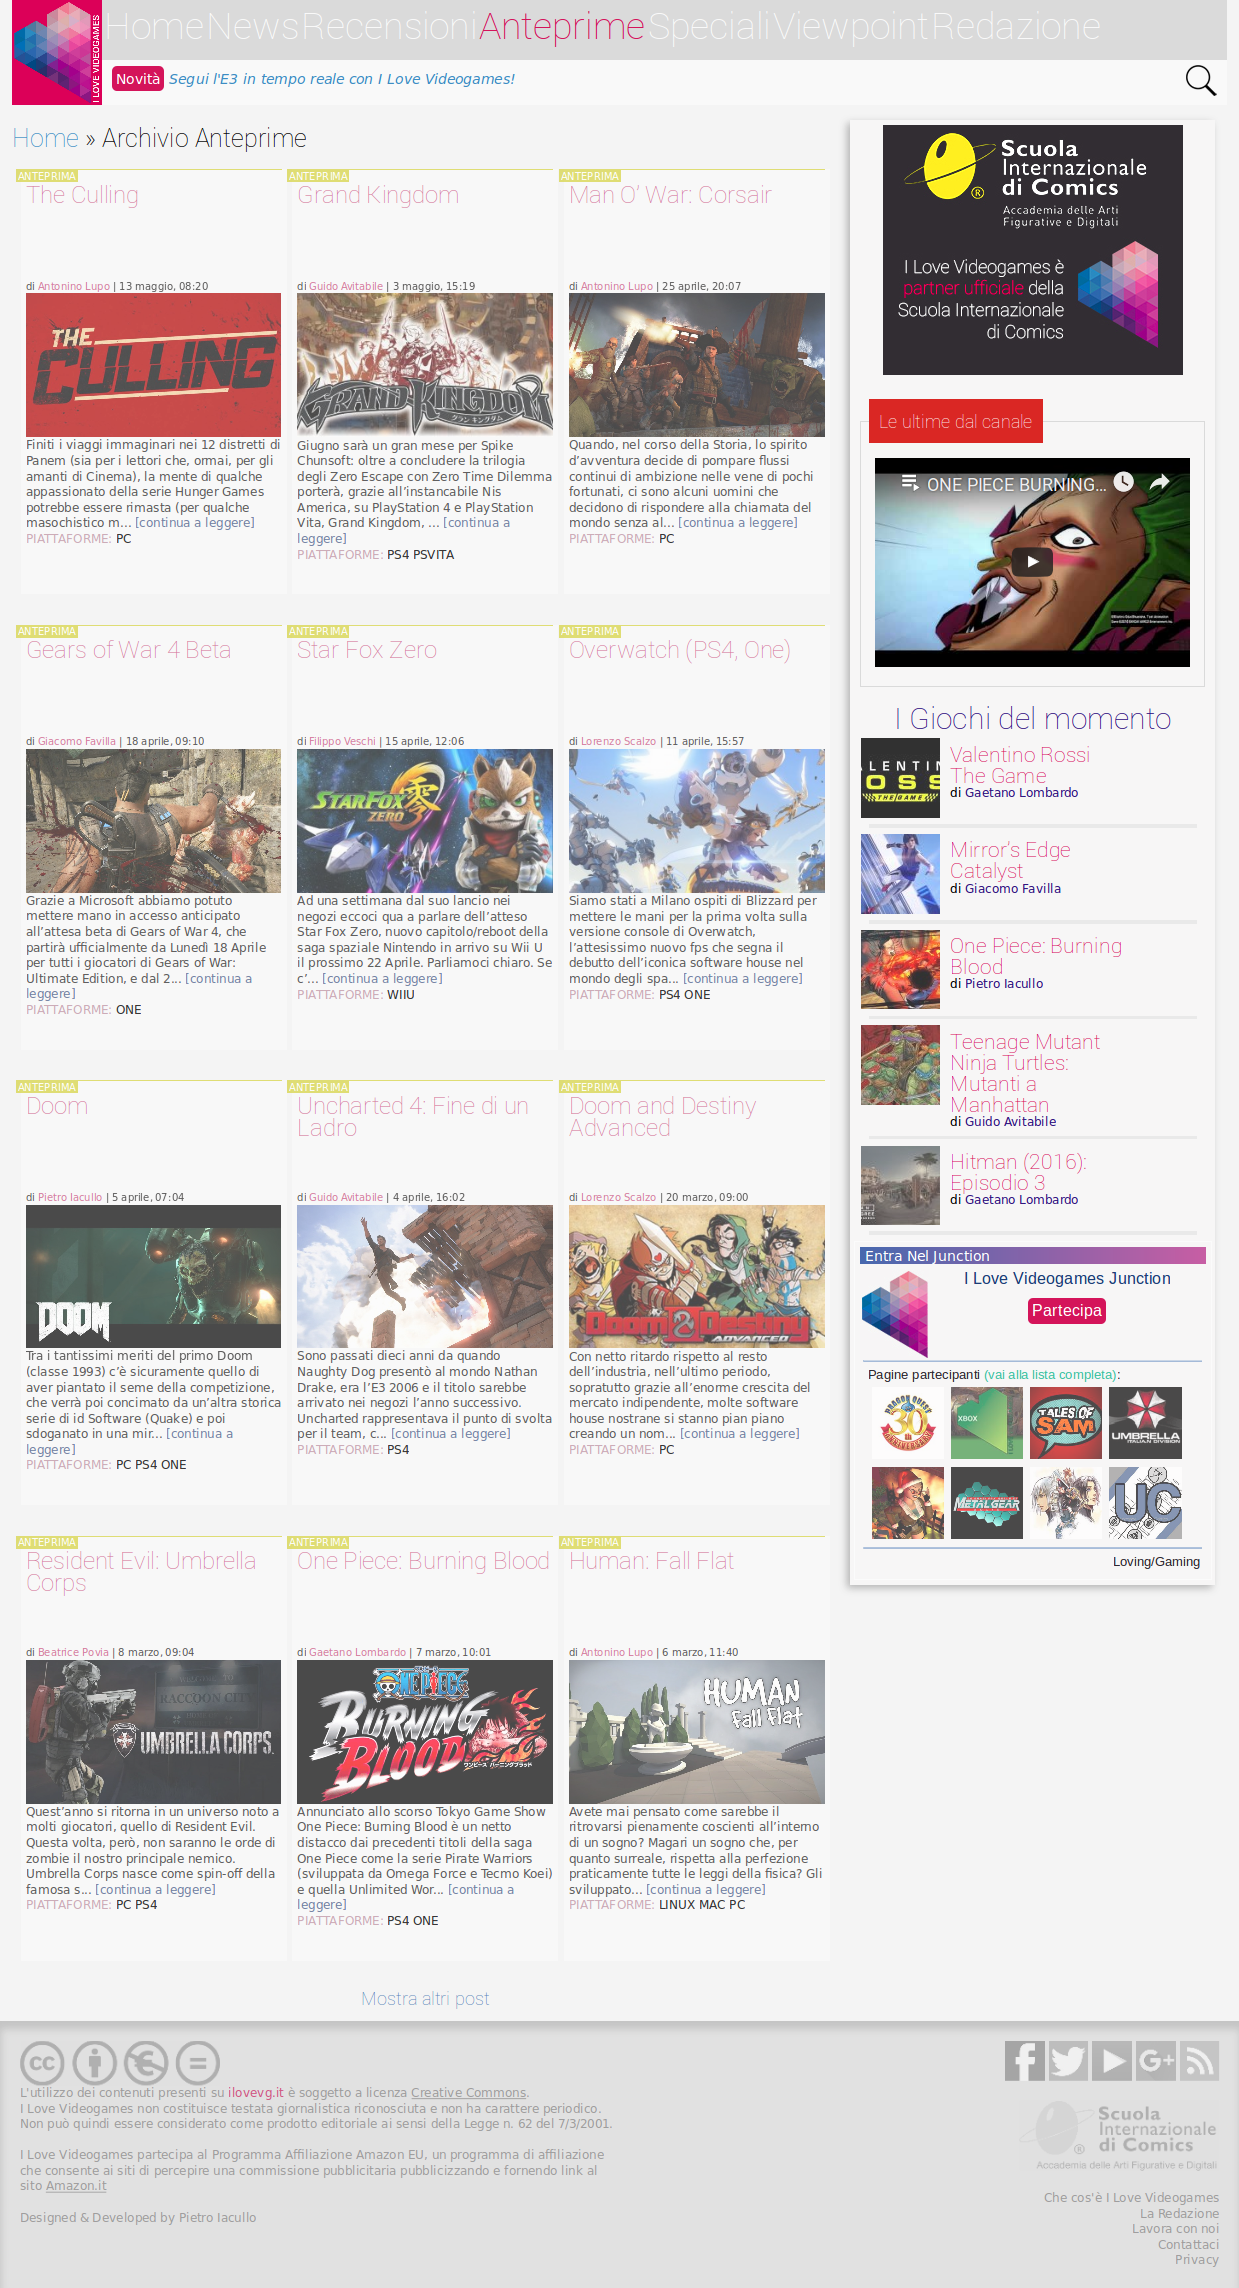
\includegraphics[scale=0.24]{img/AnteprimeCompleta}
			\caption{Pagina con l'archivio delle anteprime}
	\end{figure}

	\begin{figure} [H]
			\centering
			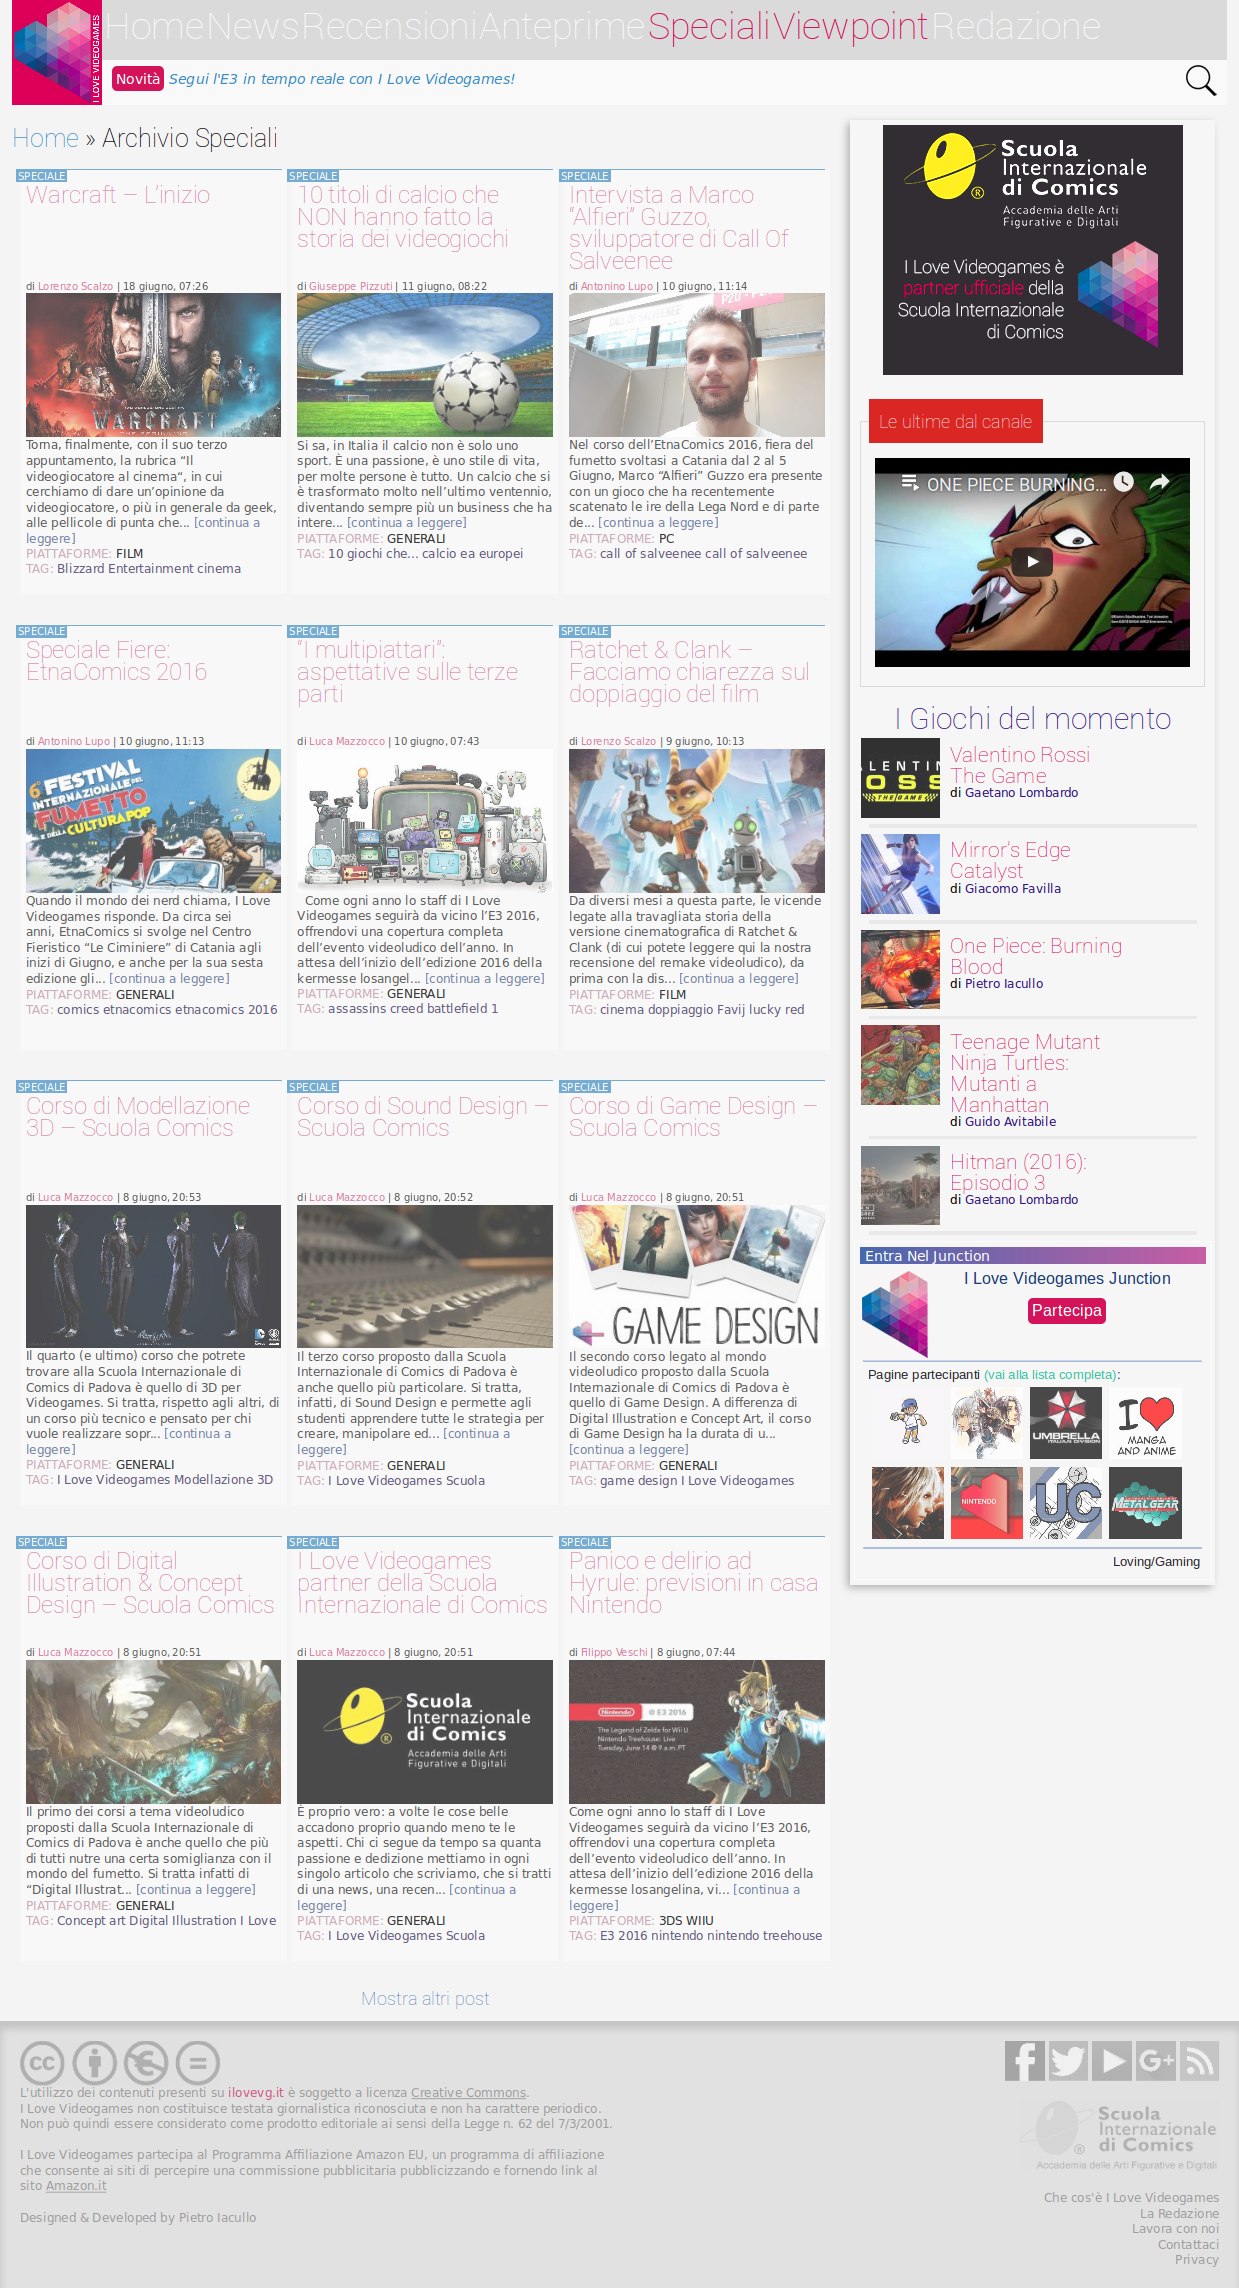
\includegraphics[scale=0.24]{img/SpecialiCompleta}
			\caption{Pagina con l'archivio dei contenuti speciali}
	\end{figure}

		\subsubsection{Considerazioni generali}
		Essendo tali pagine praticamente uguali all'home page se non per i contenuti, tutte le considerazioni fatte sull'home page valgono anche per tali pagine. L'unica nota aggiuntiva da fare riguarda i breadcrumbs di tipo location: infatti ogniuna di queste li prevede e ciò permette di capire in che pagina della gerarchia del sito ci si trova. L'aggiunta dei breadcrumbs in queste pagine è importante poichè permette di chiarificare l'asse ``where''.
		\begin{figure} [H]
				\centering
				
\includegraphics[scale=0.6]{img/BreadcrumbsNews}
				\caption{Breadcrumbs della pagina News}
		\end{figure}

	\newpage
	\subsection{Pagina di una news}
	La pagina di una news presenta una notizia del sito.
	\begin{figure} [H]
			\centering
			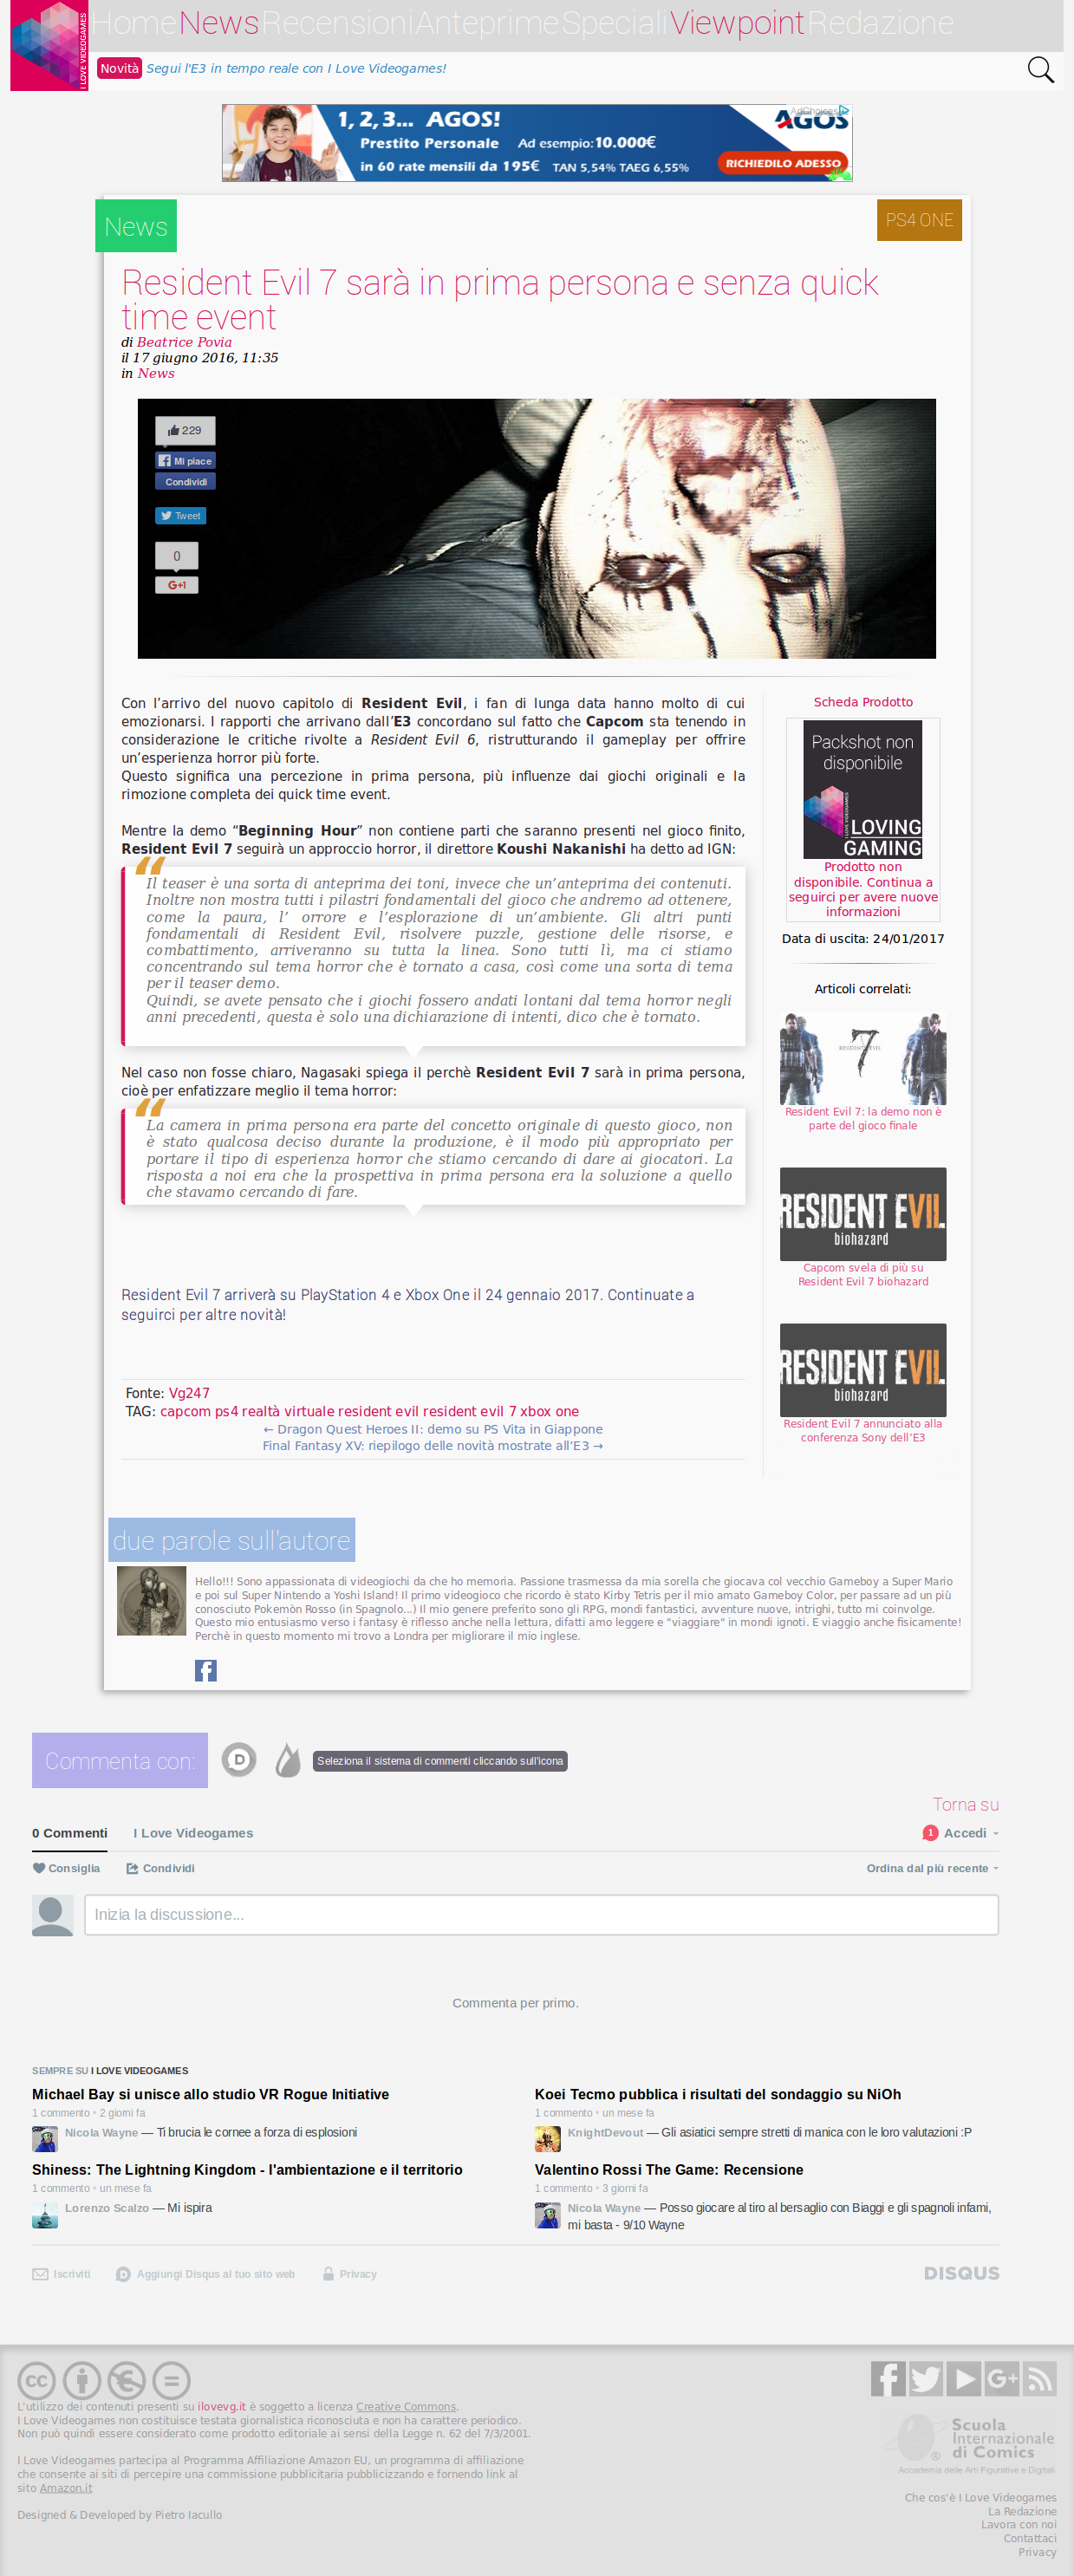
\includegraphics[scale=0.16]{img/NewsSingolaCompleta}
			\caption{Pagina di una news}
	\end{figure}
		\subsubsection{Le 6W}
			\paragraph{When}
			Asse opzionale che rappresenta le novità. Possiamo consideriamo la pagina stessa come parte dell'asse ``when''. Difatti la notizia è riportata con data e ora di pubblicazione e quindi associa una indicazione temporale al sito.

			\paragraph{Why}
			Asse opzionale consigliato che rappresenta la descrizione del sito web. Tale asse non è soddisfatto in quanto non è presente alcuna descrizione del sito web nella pagina.

			\paragraph{How}
			Asse opzionale consigliato che rappresenta il modo in cui è possibile muoversi all'interno del sito web. Tale asse è soddisfatto dalla search box che compare faccendo un click sulla lente di ingrandimento in alto a destra. La posizione scelta è la migliore infatti gli utenti sono abituati a trovare in quel punto la search box. 
			
			\paragraph{Who}
			Asse obbligatorio che descrive chi rappresenta il sito. Tale asse è pienamente soddisfatto dal logo posizionato in alto a sinistra accompagnato dal nome del sito web. La scelta di questa posizione è la migliore per gli utenti.

			\paragraph{What}
			Asse obbligatorio che serve dire all'utente cosa il sito propone. Tale asse è soddisfatto dalla presenza del menù nella parte alta della pagina, il quale presenta un link diretto alla Home.

			\paragraph{Where}
			Asse obbligatorio che indica all'utente doce si trova all'interno del sito. Tale asse è soddisfatto solo parzialmente. Questo perchè il sito, in questo tipo di pagine, non propone alcun tipo di breadcrumbs. L'unica indicazione di dove ci si trova viene data dal menu: viene infatti colorata la scritta ``News''.

		\subsubsection{Considerazioni generali}
		Nella parte iniziale della pagina troviamo un'immagine molto grande connessa alla notizia. Una migliori potrebbe esssere ridurre la dimensione di tale immagine lasciando più spazio al testo (comunque più importante nel web rispetto le immagini) e limitando così lo scroll. Questa immagine inoltre non è cliccabile. La pubblicità nel top della pagina anche aumenta lo scroll ed inoltre non potrebbe sfruttare l'effetto blending: le pubblicità che mi sono state proposte erano di Agos, Zalando e Infostrada mentre in un sito di videogames mi aspetterei di trovare o pubblicità di videogiochi o di comunque qualcosa di inerente a questo mondo: console, computer o al massimo tecnologia in generale. \\

		Molto positivo è dare la possibilità di condividere la notizia su Facebook, Twitter e Google+, come dare la possibilità di mettere ``Mi piace'' direttamente dalla pagina e di lasciare un commento. Positivo è anche che nella parte sinistra della pagina ci siano link a notizie correlate: se un utente è interessato alla notizia potrebbe voler leggere qualcosa di correlato e grazie a queste proposte è possibile aumentare il tempo che un utente passa sul sito web. Infine è sempre una bella idea il fatto che in fondo alla pagina ci sia la sezione ``Due parole sull'autore'' che propone una autodescrizione dell'autore ed il link alla sua pagina Facebook.

	\newpage
	\subsection{Pagina di una recensione}
	La pagina di una recensione presenta la recensione un videogame.
	\begin{figure} [H]
			\centering
			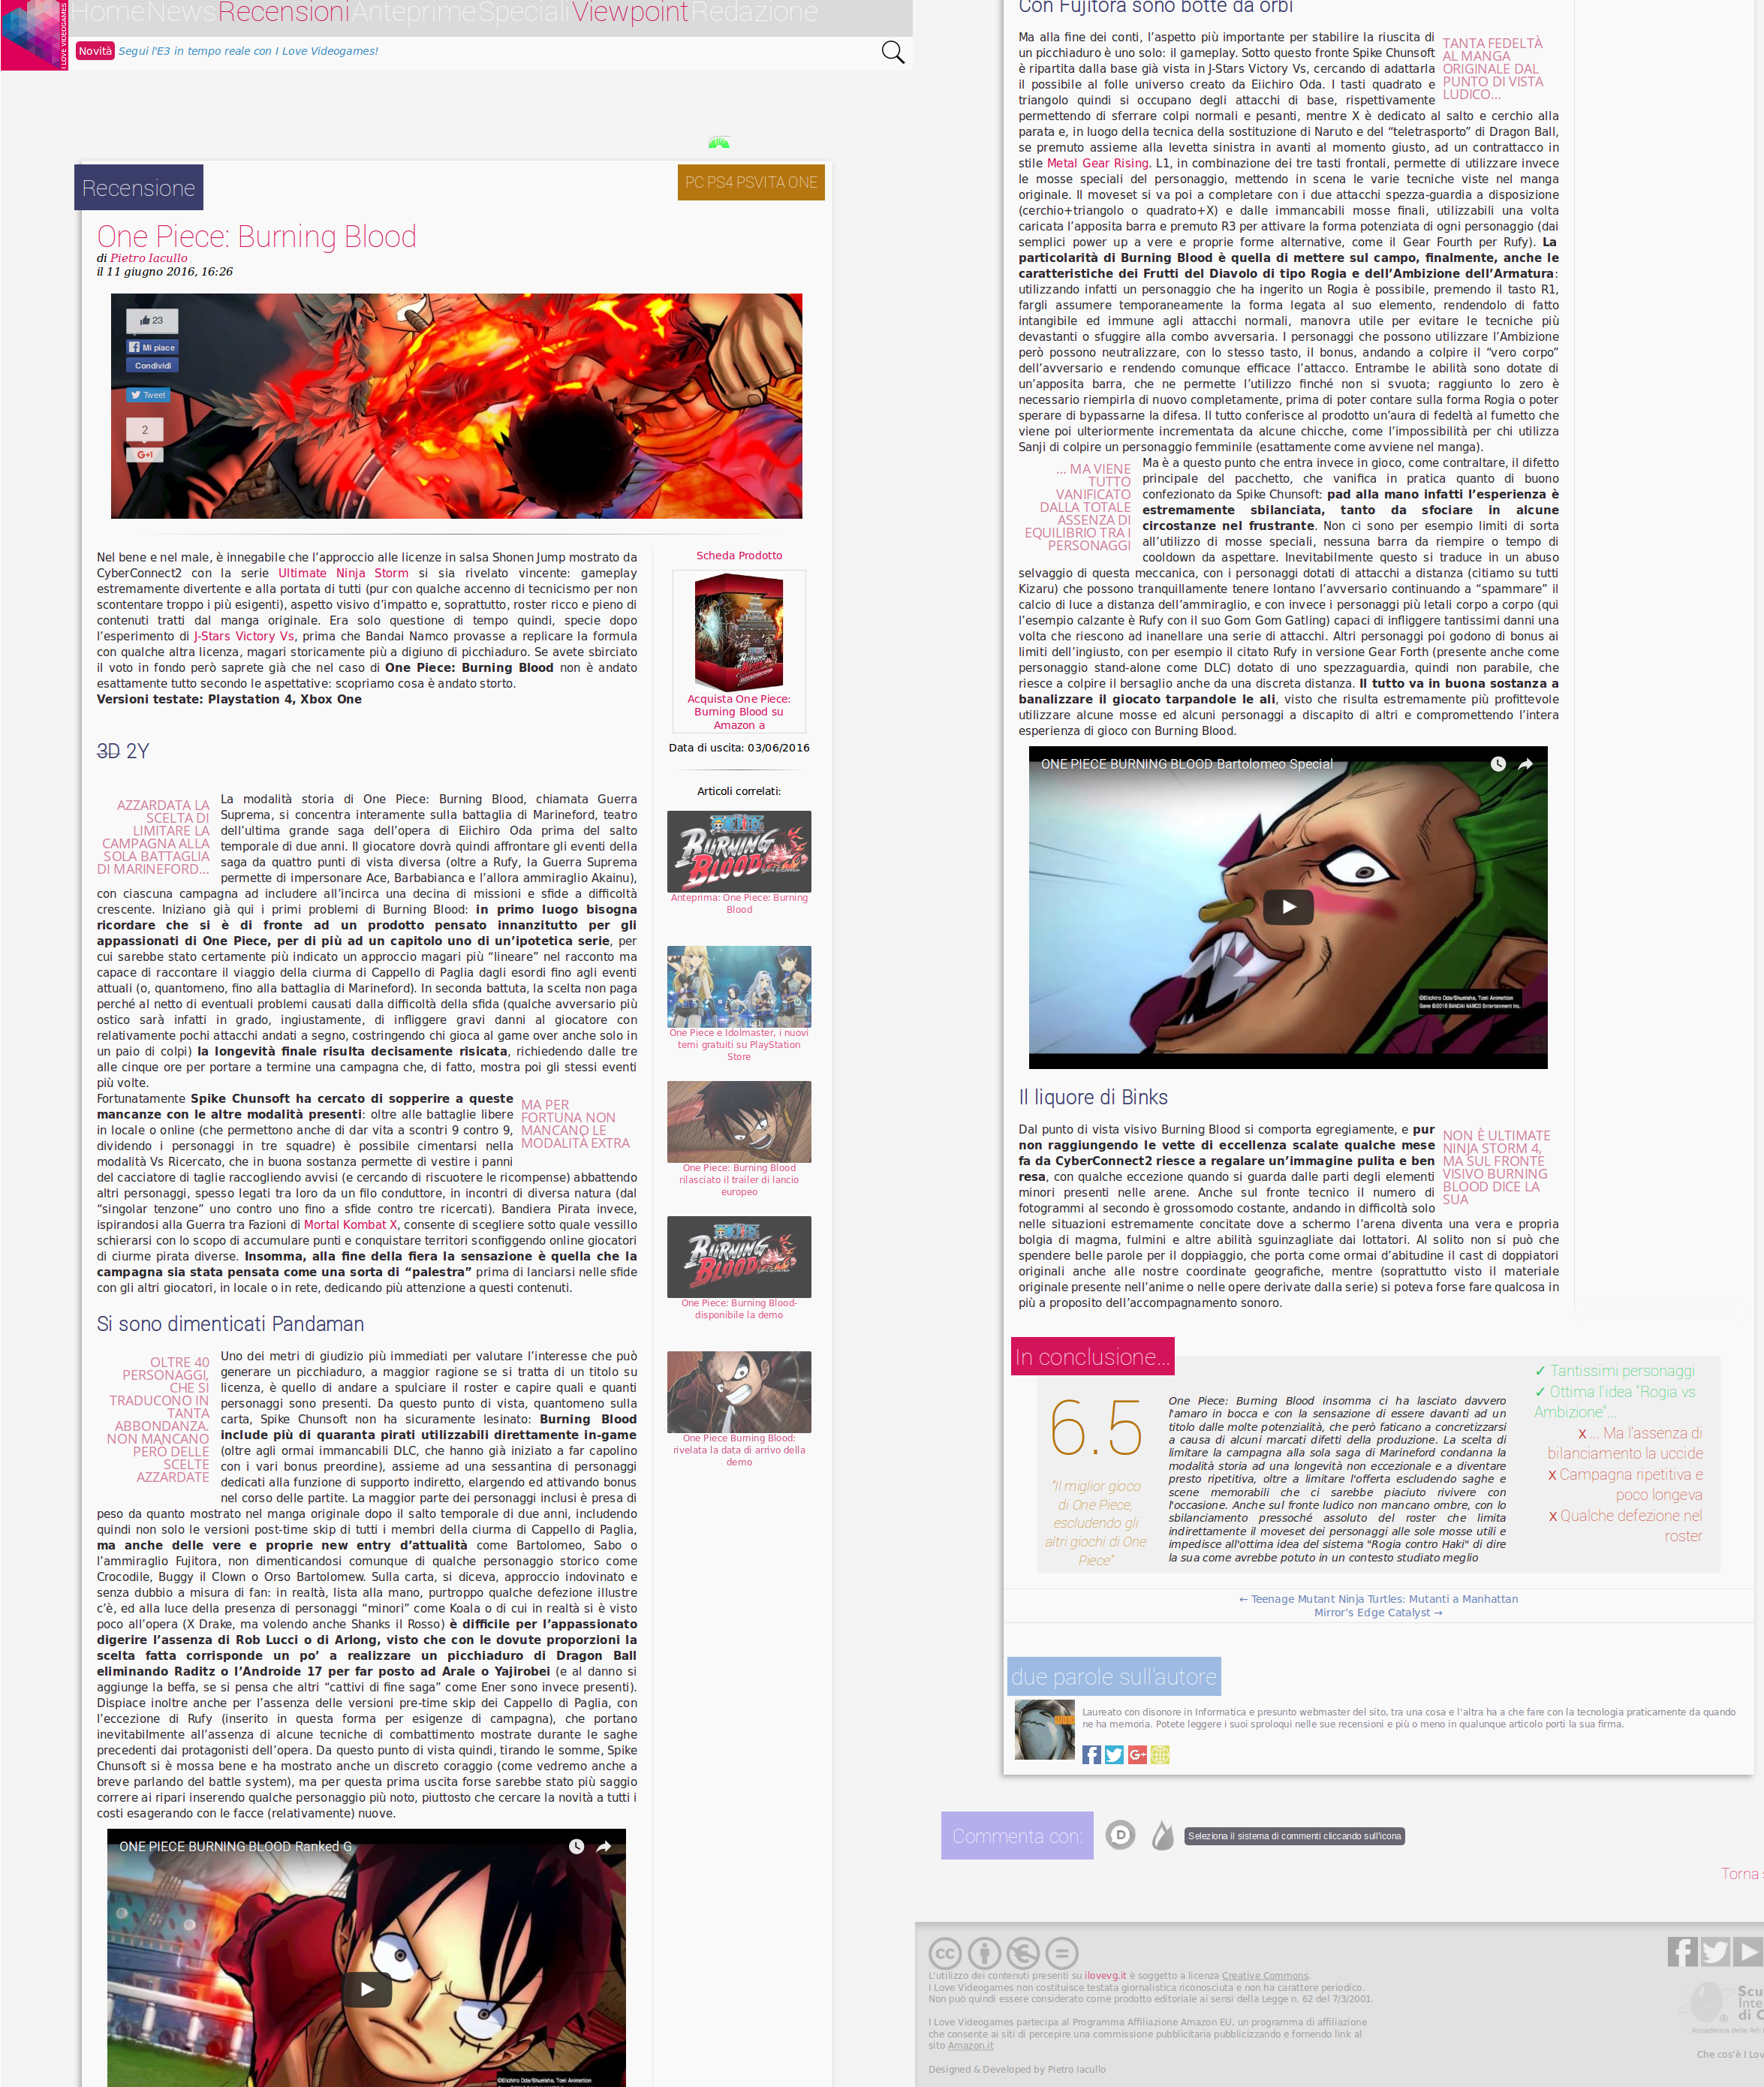
\includegraphics[scale=0.15]{img/RecensioneSingolaCompleta}
			\caption{Pagina di una recensione}
	\end{figure}
		\subsubsection{Le 6W}
		La struttura della pagina è uguale rispetto alla pagina che presenta una specifica notizia. Di conseguenza le considerazioni riguardanti le 6W rimangono inalterati rispetto tale pagina.

		\subsubsection{Considerazioni generali}
		Mantenendo la stessa struttura anche le considerazioni generali saranno simili a quelle della pagina che presenta una news. A tali consideerazioni c'è da aggiungere che in questo caso lo scroll può essere veramente eccessivo (l'immagine di esempio della pagina infatti è dovuta essere ritagliata per motivi di spazio) soprattutto nel caso di videogiochi valutati molto positivamente dal sito. Positivo invece è l'inserimento di video relativi al videogioco recensito, che danno completezza alla recensione, e la struttura del testo. Il testo è organizzato in sezioni divise da titoli e presenta parole chiave evidenziate in grassetto: il problema è che talvolta sono evidenziate frasi intere. Inoltre alla fine della recensione è presenta una sezione che riassume la recensione, interessante per un utente che vuole sapere un'opinione senza leggersi tutti il testo.
		\begin{figure} [H]
			\centering
			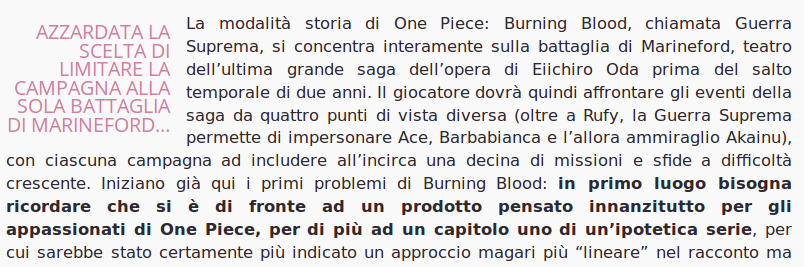
\includegraphics[scale=0.4]{img/ErratoUsoGrassetto}
			\caption{Esempio di errato uso del grassetto}
		\end{figure}

	\subsection{Pagine di una anteprima e di uno speciale}
	Tali pagine presentano rispettivamente la recensione di un videogioco in uscita e per presentare un contenuto del sito che non rientra nelle altre categorie o che deve essere messo in evidenza.

		\subsubsection{Considerazioni generali}
		Queste pagine sono del tutto simili nella struttura alle pagine sopra analizzate e quindi non ne è stata fatta una descrizione specifica ma sono state citate per completezza.
	\begin{figure} [H]
		\centering
		\includegraphics[scale=0.18]{img/AnteprimaSingolaCompleta}
		\caption{Pagina di una anteprima}
	\end{figure}
	\begin{figure} [H]
		\centering
		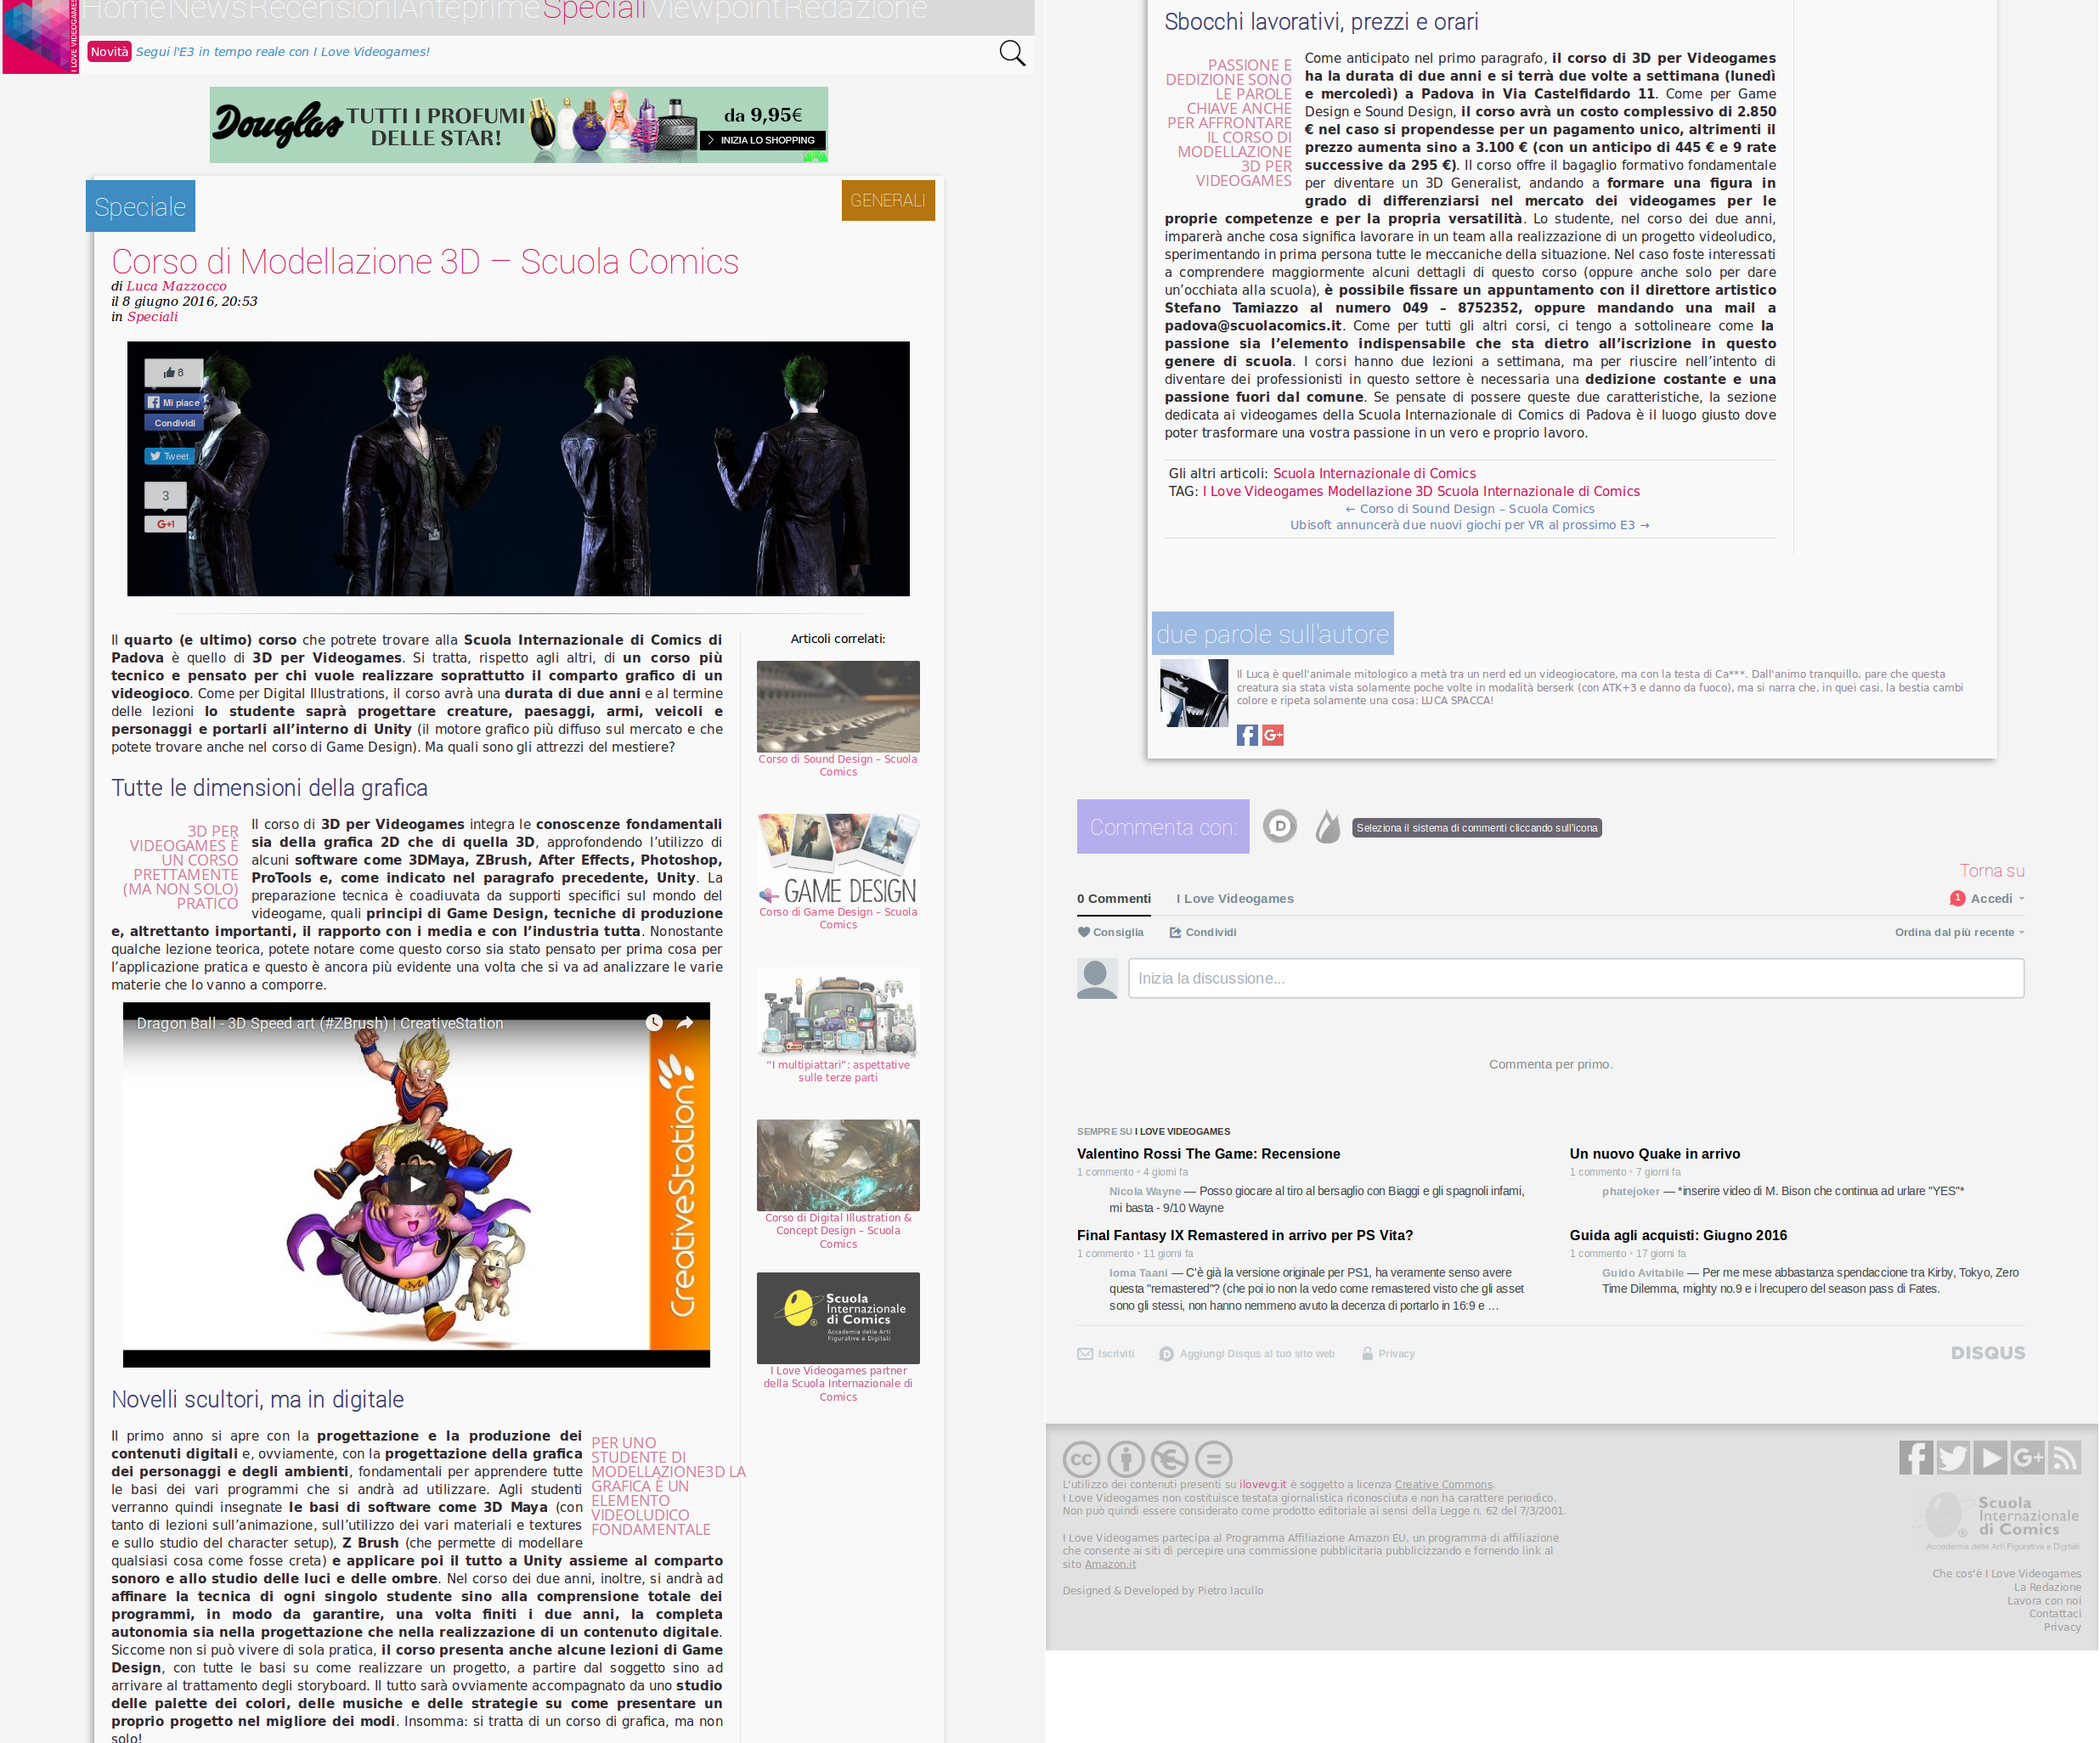
\includegraphics[scale=0.18]{img/SpecialeSingolaCompleta}
		\caption{Pagina di uno speciale}
	\end{figure}

	\newpage
	\subsection{Pagina della redazione}
	La pagina della redazione presenta le persone che contribuiscono al sito web.
	\begin{figure} [H]
			\centering
			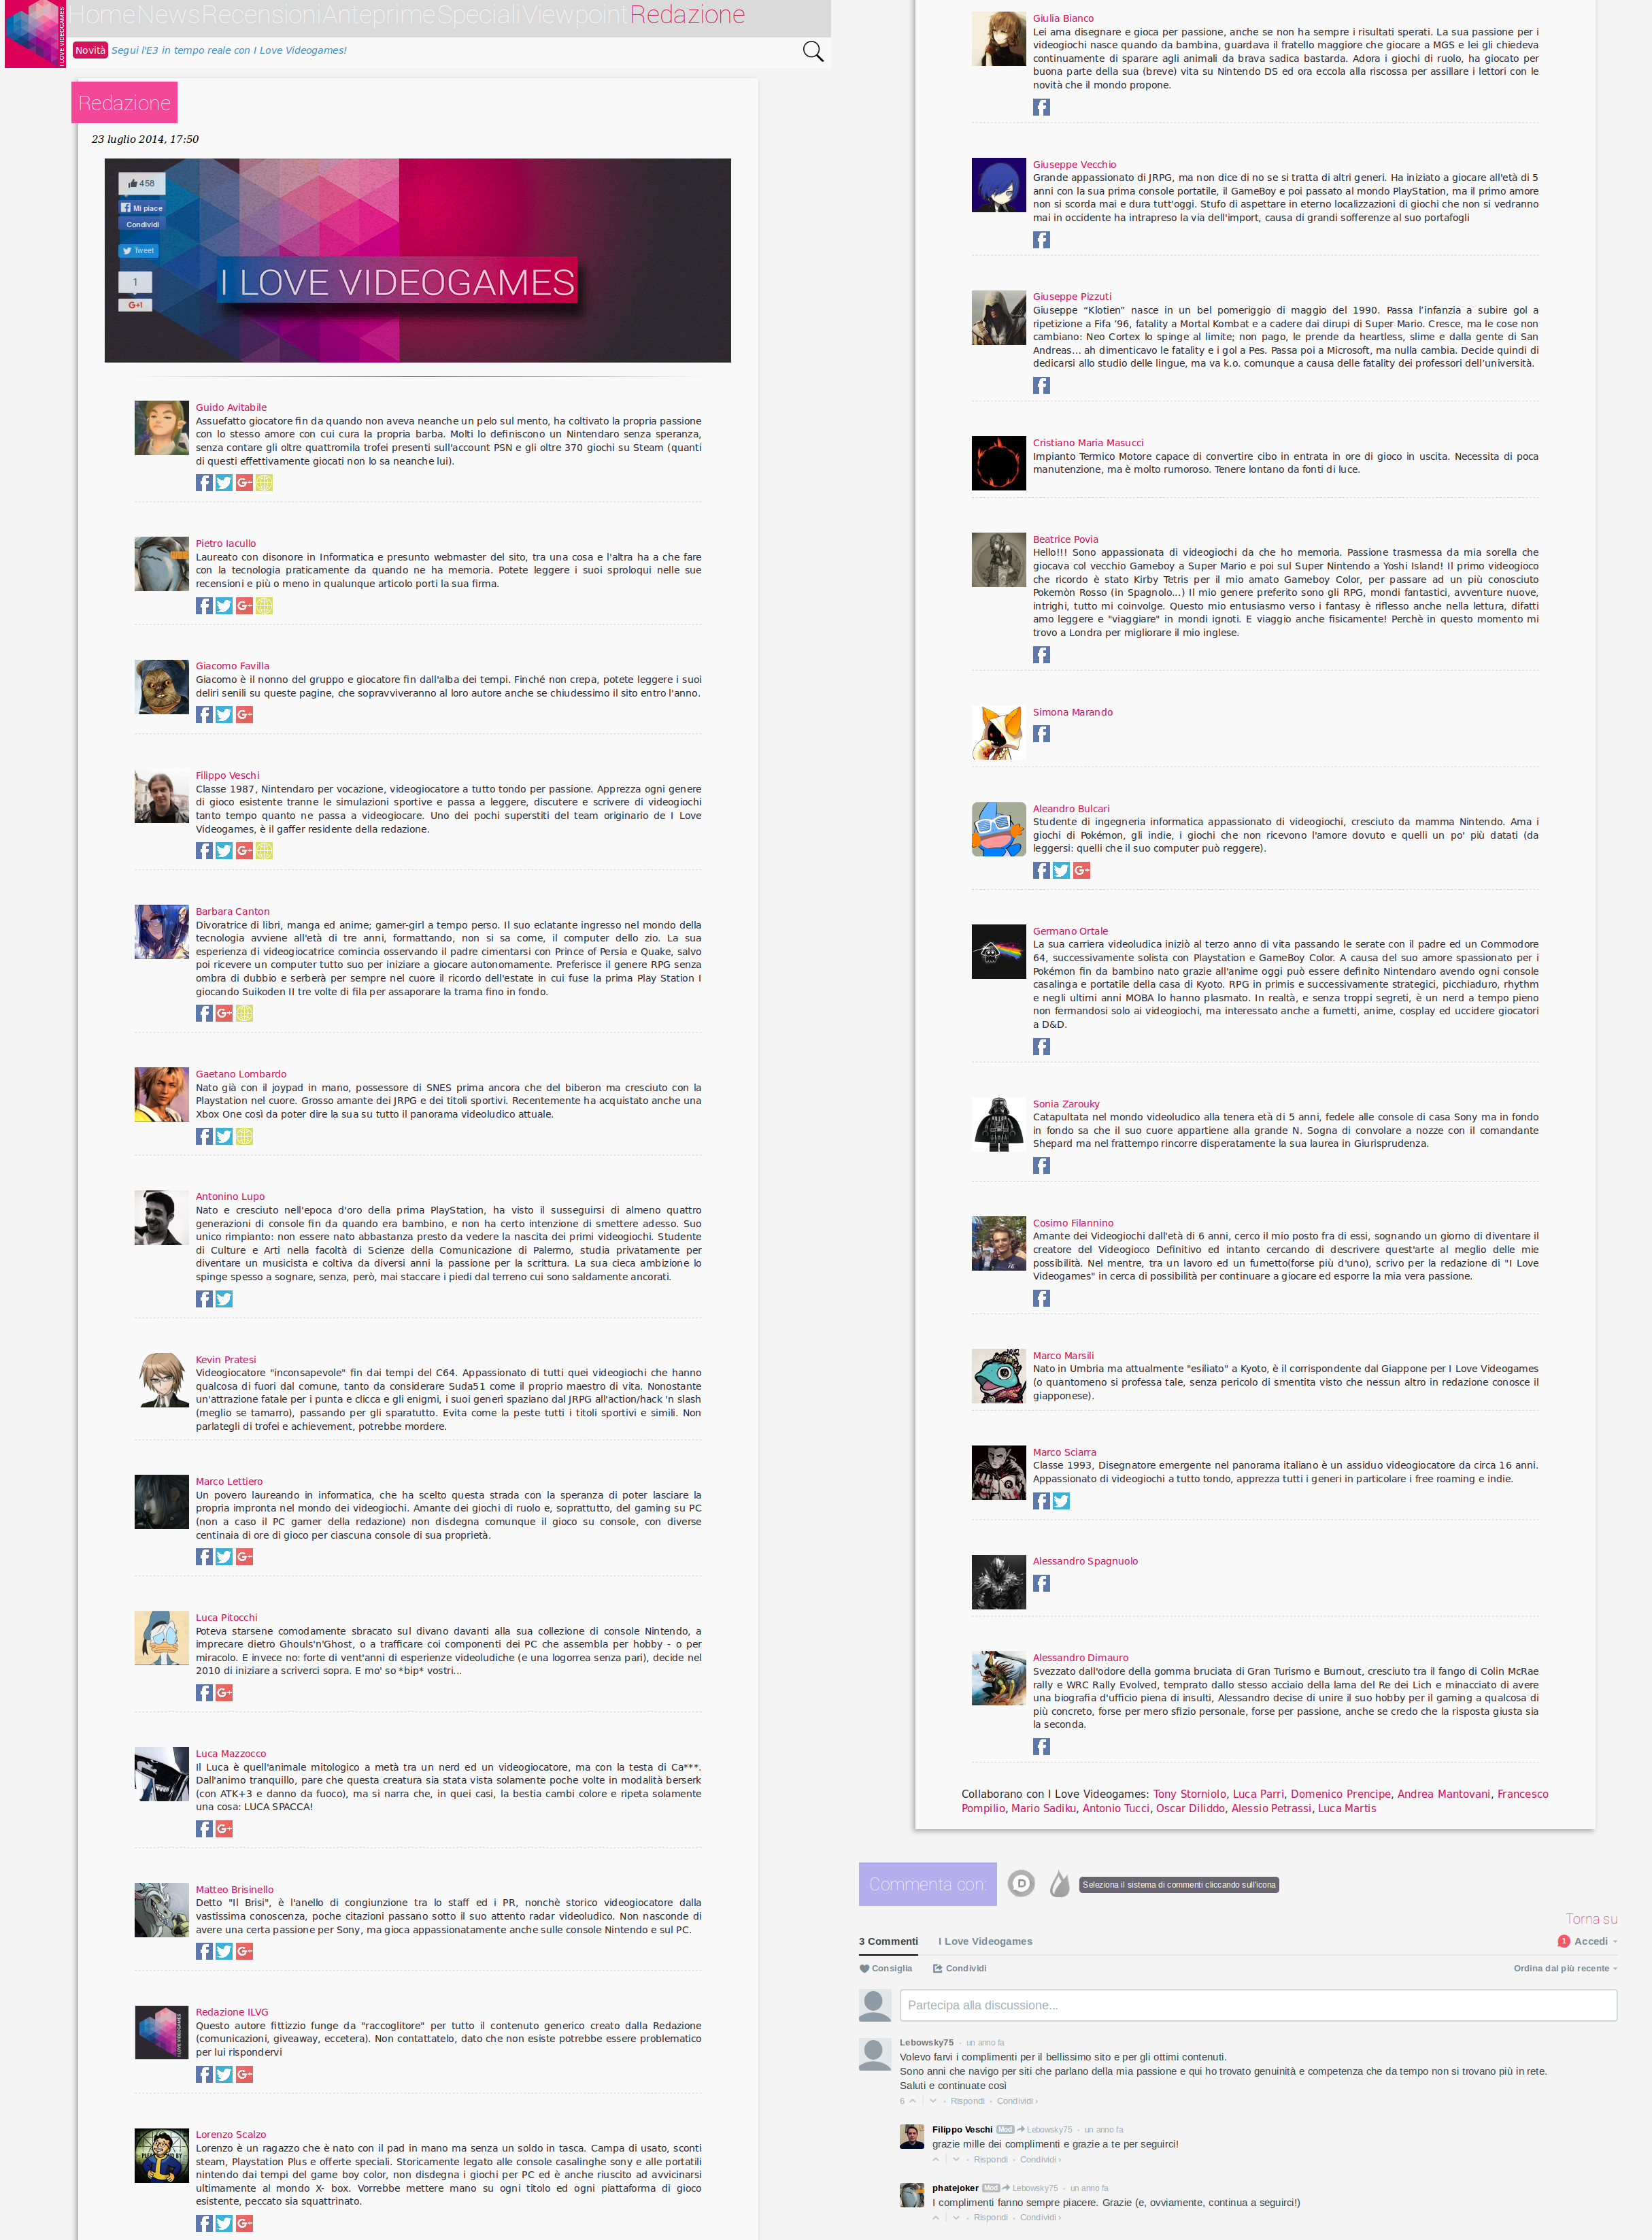
\includegraphics[scale=0.15]{img/Redazione}
			\caption{Pagina della redazione}
	\end{figure}
		\subsubsection{Le 6W}
		Pur mantenendo una struttura simile alle altre pagine interne questa pagina presenta delle differenze.

			\paragraph{When}
			Tale asse è poco sviluppato. Difatti viene solamente riportata una data in cima alla pagina che non si capisce se è la data di creazione della pagina o dell'ultima modifica. Potrebbe essere stato utile per sviluppare tale asse inserire le date in cui i vari collaboratori hanno iniziato a lavorare al sito, dando cosi ulteriori informazioni agli utenti.

			\paragraph{Why}
			Questo asse è quasi del tutto assente. L'unico elemento rimandabile alla descrizione del sito è la grande immagine presente all'inizio della pagina.

			\paragraph{How}
			L'asse ``how'' è soddisfatto, come le altre pagine dalla search box posizionata in altro a destra.
			
			\paragraph{Who}
			Tale asse risulta essere quello, ovviamente, più sviluppato. Infatti questa pagina presenta appunto le persone che lavorano al sito. È sempre presente in alto a sinistra il logo del sito ed una parte del logo è richiamata anche nell'immagine in alto nella pagina.

			\paragraph{What}
			Come nelle altre pagine tale asse è soddisfatto grazie alla presenza del menù nella parte alta della pagina, che prevede un link alla Home.

			\paragraph{Where}
			Questo asse può essere considerato soddisfatto grazie al menù che indica in quale sezione del sito ci troviamo.
		
		\subsubsection{Considerazioni generali}
		Questa pagina come le altre prevede uno scroll verticale eccessivo, anche se in questa pagina è più tollerabile: gli utenti la dovrebbero visitare raramente e, inoltre, potrebbe essere spiacevole relegare qualche persona che lavora al sito in una pagina secondaria. Anche qui troviamo i link agli account sui maggiori social di quasi tutti i collaboratori facenti parte della redazione, corredati da una breve e ironica presentazione. L'idea di questa pagina di presentazione avrebbe potuto avere ancora più effetto, secondo me, utilizzando delle foto reali invece che immagini di personaggi di videogiochi, film o fummetti poichè potrebbe scatenare in un utente ancora più simpatia verso il sito vedere chi ci lavora. Anche in questo caso l'immagine nella parte alta della pagina è troppo ingombrante.
\end{document}
